
\runningheader{Oppgave o)}{}{Side \thepage\ av \numpages}


% ********************************************************
% oppgave o) 
% ********************************************************  
\item[o)]
   Kjør først filen \fbox{\tt oving2\_data.m}, og lag deretter
   modellen vist under
  \begin{figure}[H]
    \centering
    \hspace*{0mm}\scalebox{0.8}{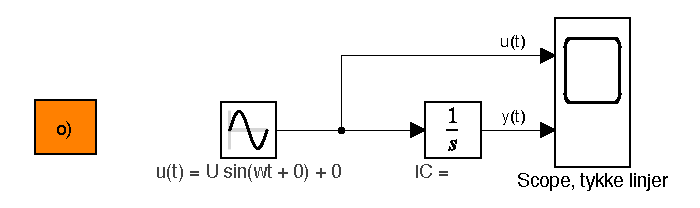
\includegraphics{2o.pdf}}
  \end{figure}
  Som du ser har vi spesifiser $u(t)$ som
  \begin{align}
    \label{eq:1ew}
    u(t) & = U \sin(\omega {\cdot}  t)
  \end{align}
  hvor $U{=}0.5$ og $\omega {=} 0.3$ rad/s gitt i .m-filen.
  Ved å integrere $u(t)$ med initialverdi $y(0){=}0$ finner vi uttrykket
  for $y(t)$ som
  \begin{align}
    y(t)  & = -\frac{U}{\omega}{\cdot}\cos(\omega{\cdot}t) +  \frac{U}{\omega}\label{eq:7aaa}
  \end{align}
  {\color{red}La simuleringstiden nå være 100 sekund, og ikke 25
    sekund som tidligere.  }

  {\bf Gjør følgende oppgaver / svar på følgende spørsmål:    }
  
\begin{enumerate}[label=o\arabic*)]
  \item Sett initialverdien til {\sf 0} i integratoren.
 Simuler modellen og 
    vis at responsen til $y(t)$ alltid er større enn 0. Gi en
    forklaring på hvorfor det er slik.    
    Ta med simuleringsresulatet
    i innleveringen din ved å bruke prosedyren på
     side~\pageref{page:prosedyre}.

  \item   Vi ønsker å få $y(t)$-kurven til å 
  svinge omkring $y{=}0$, og den eneste måten å få dette til på er å
  redusere initialverdien $y(0)$ i integratoren. Bestem ny
  initialverdi som gjør at $y(t)$ svinger omkring $y{=}0$, og simuler på ny.
    Ta med simuleringsresulatet
    i innleveringen din.
  
 

  \end{enumerate}
